\documentclass{beamer}


% Preamble for english writing
\usepackage[utf8]{inputenc}
\usepackage[T1]{fontenc}
\usepackage{amsmath}
\usepackage{amsfonts}
\usepackage{amssymb}
\usepackage{amsthm}
%\usepackage{algorithmic}
\usepackage{color}
\usepackage{enumerate}
\usepackage{stmaryrd}
\usepackage{hyperref}
\usepackage{graphicx}

%\usepackage{tkz-graph}

%\usepackage[nottoc, notlof, notlot]{tocbibind}

%%%%%%%%%%%%%%%%%%%%%%%%%%%%%%%%%%%%%%%%%%%%%%%%%%%%%%%%%%%%%%%%%%%
%Commandes ajoutées
%%%%%%%%%%%%%%%%%%%%%%%%%%%%%%%%%%%%%%%%%%%%%%%%%%%%%%%%%%%%%%%%%%%

%ensmembles
\newcommand{\N}{\mathbb{N}}
\newcommand{\Z}{\mathbb{Z}}
\newcommand{\Q}{\mathbb{Q}}
\newcommand{\R}{\mathbb{R}}


\newcommand{\intv}[2]{\llbracket #1, #2 \rrbracket} %intervalle d'entiers
\newcommand{\bracket}[1]{{\langle #1 \rangle}} %parenthèses angulaires
\newcommand{\gO}{\mathcal{O}} %grand O
\newenvironment{itemiz}{\renewcommand\labelitemi{$\blacktriangleright$}\begin{itemize}}{\end{itemize}}

\newcommand{\rg}{\text{rg}}
\newcommand{\bad}{\textbf{/!\backslash}}

\newcommand{\crk}{\text{cut-rank}}

\newcommand{\ie}{\emph{i.e.}\ }
\newcommand{\eg}{\emph{e.g.}\ }
\newcommand{\cf}{\emph{c.f.}\ }

% Theorems etc.
\newtheorem{Thm}{Theorem}[section]
\newtheorem{Cor}[Thm]{Corollary}
\newtheorem{Lem}[Thm]{Lemma}
\newtheorem{Pro}[Thm]{Proposition}

\theoremstyle{remark}
\newtheorem{Rem}[Thm]{Remark}
\newtheorem{Not}[Thm]{Notation}
\newtheorem{Exa}[Thm]{Example}

\theoremstyle{definition}
\newtheorem{Def}[Thm]{Definition}

\newcommand{\mytitle}[1]{
\begin{center}
\vspace{7cm}
\hrule
\vspace{0.5cm}
\huge{\textsc{#1}}
\vspace{0.5cm}
\hrule
\vspace{1cm}
\end{center}}



\usepackage{wallpaper}
%\usecolortheme{beaver}
\usetheme{Berlin}



\title{\textbf{Evolutionary Computing \\on Turing Machines}}
\subtitle{Solving the Busy Beaver Problem}
\author{Jean-Florent Raymond \and Emilio Del Tessandoro}
\institute[Uppsala University]{Uppsala University}
\date{\today}




\begin{document}

{
	%I have to put it here otherwise goes on every page!
	\usebackgroundtemplate{%
		\vbox to \paperheight{\vspace{5cm}\hbox to \paperwidth{\hfil
\includegraphics[width=3cm]{figures/uu_logo_transparent.png}\hfil}}
	}
	
	\begin{frame}
	\titlepage
	\end{frame}
}
\section{Introduction}

\begin{frame}
\frametitle{What Is a Turing Machine?}
\begin{columns}[c]
	\begin{column}{5.5cm}
		\begin{figure}
		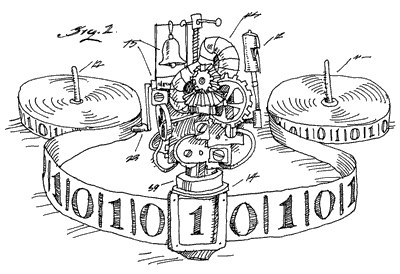
\includegraphics[width=5.5cm]{figures/turingMachine.png}
		\end{figure}
	\end{column}
	\begin{column}{6cm}
		Is an \textbf{hypothetical device} with:
		\begin{itemize}
		\item an internal state $S \in Q$
		\item an infinite tape (symbols in $\Sigma$)
		\item a transition function $\delta$
		\end{itemize}
		
		\[\delta : Q \times \Sigma \to Q \times \Sigma \times \{L,R\}\]
	\end{column}
\end{columns}
\end{frame}


\begin{frame}{The Busy Beaver Problem}

\end{frame}

\begin{frame}{Why It Is So Hard}

\begin{itemize}
\item The size of the search space is exponential in the size of the machines;
\item $S$ grows extremely fast, even faster than the search sapce;
\item Because of the halting problem, $S$ is not computable;
\item How the halting machines are distributed is not known and not easy.
\end{itemize}
\end{frame}

\begin{frame}{Why It Is So Hard, Continued}


\only<1>{
\framesubtitle{Order of magnitude of the search space}

\begin{center}
\begin{tabular}[h!]{|c|c|c|c|c|}
  \hline
    & 2 symbols & 3 symbols  & 4 symbols\\
  \hline
  2 states&$10^4$ &$10^7$   &$10^{17}$\\
  \hline
  3 states&$10^7$ &$10^{12}$ &$10^{18}$\\
  \hline
  4 states&$10^8$ &$10^{17}$ &$10^{25}$\\
  \hline
\end{tabular}
\[
\left (2 \times M \times(N+1) \right ) ^{MN}
\]
\end{center}
}\only<2>{
\framesubtitle{Values and lower bounds for $S$ (max step function)}

\begin{center}
\begin{tabular}[h!]{|c|c|c|c|c|}
  \hline
          & 2 symbols & 3 symbols  & 4 symbols\\
  \hline
  2 states&6          &38          &$>10^6$\\
  \hline
  3 states&21         & $> 10^{17}$ &$>10^{13036}$\\
  \hline
  4 states&107        &$>10^{14072}$ &?\\
  \hline
\end{tabular}
\end{center}
}
\end{frame}

\section{Possible Solutions}

\begin{frame}{Other Approaches}

\begin{itemize}
\item Naïve method : run different machines and keep to one who halts after the more steps ; %improved if we detect loops
\item Detect patterns on the tape to predict future action.
\end{itemize}

\end{frame}

\begin{frame}{Our Approach}
\framesubtitle{A Genetic Algorithm}

\begin{itemize}
\item on a population of Turing machines;
\item operations : mutation, crossover;
\item fitness:
  \begin{itemize}
  \item 0 if $S$ is overtaken ;
  \item inverse of distance to the $S$ else.
  \end{itemize}
\item fitness of 1 means that we found a busy beaver.
\end{itemize}

\end{frame}

\begin{frame}{What We Did}

%C++ implementation, TM virtual machine and the EC tool
\begin{enumerate}
\item we did a C++ imlementation :
  \begin{itemize}
  \item program to handle and run TM ;
  \item genetic algorithm.
  \end{itemize}
\item we run tests ;
\item we get results.
\end{enumerate}
\end{frame}

\section{Results}

\begin{frame}{What We Found}
Busy beavers for the instances (2,2), (2,3), (3,2) and (2,4)
\end{frame}

\begin{frame}{Actual Results}
% we found all known busy beavers
Busy beavers for the instances (2,2), (2,3), (3,2) and (2,4)
\end{frame}

\section{Conclusions}

\begin{frame}{Conclusions}
Using a genetic algorithm made us able to find all currently known busy beavers much more faster than using bruteforce.
Solving the other cases seems impossible with our current implementation, but we have a lot of optimization ideas.
\end{frame}

\end{document}